
\subsection{Overview}
After the problem statement and an brief description of Simian tool, we go to describe a possible approach to solve the problem of API function call recommendations. This approach, described in Figure 2, exploits the CLAMS work, in particular the patterns extracted as output, plus the code cloning features provided by Simian. So, at the beginning of the process and after a preprocessing phase, we have the patterns files and the developer's file, represented by a single string. Notice that with this way we keep trace on the context in which the user is developing. Then, all these files is used to extract the recommendations in form of patterns by using Simian integrated in Eclipse platform, following the options specified in next sections. Basically, at the end of this phase, Simian retrieves the cloned clone between the developer's file and the CLAMS patterns related to the library that the user is implemented. By using these file, the tool performs recommendations by remove the cloned part and suggest to the user the new lines of code that represent the missing pattern for the user. In next sections, we going in deep to describe the entire system and how the integration of Simian and CLAMS works in practise. 


\begin{figure}[H]
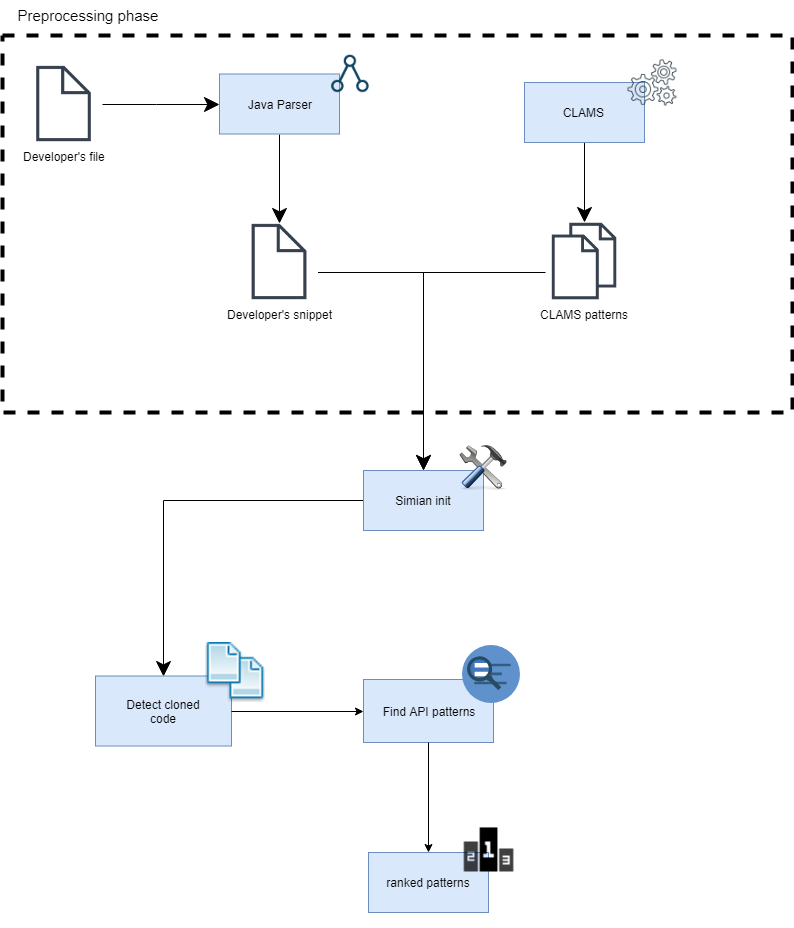
\includegraphics[width=14cm,height=16cm,keepaspectratio]{images/simian.png}
\centering
\caption{Overview of the proposed approach}
\label{fig:cmd}
\end{figure}

\subsection{Preprocessing}

About input files that are necessary to initialise the tool, we have from one side the developer's file with the real snippet of code that he is implementing and may want support for this. From the original file, we extract a portion that represent the context of the recommendation that can be a list of method invocations or simply a list of variable declaration. This portion is called ground truth and it is the part used as the context of the recommendation. On other hand, there are patterns mined by CLAMS, in form of ranked Java files sorted by rational specified in CLAMS paper. These file contains patterns, defined as sequence of API method calls that define, instantiate and using class belonging to the APIs contained in the developer' string. The number of these file and also their dimensions in term lines of code depend on the considered libraries. As Simian is a tool based on file comparison, we use temporary files of Java to do the comparison; after the process, the files are destroyed to reduce the amount of the space. \\
This preprocessing phase is required for Simian because, as we have seen in the related section, the tool not include any built-in preprocessing. To extract the snippet of code from the developer's file, we use Java parser,an open source project that allow to analyze, modify and generate Java code, to visit the AST of the input file and take the body of a method randomly selected that composes our ground truth. Notice that we consider only compilable files, otherwise Java Parser is not able to build the corresponding AST for the analysis. We take into consideration only the ground truth file because we are in the typical scenario in which the developer is starting to implement some features, so it writes only fragments of code, with a maximum length of 10 lines of code. Reversely, we don't consider an entire class or project, because in this scenario, the developer has completed almost the task and it is not interest in possible recommendations. 
As said before, in general a recommendation relies on the context in which the developer is implementing features. In our case, the context is the developer's code snippet with imports and variable declarations.\\
About CLAMS pattern, we create a golden set of 5 libraries, chosen among the 15 libraries provided by the authors on the website; for each of them, CLAMS retrieves a list of pattern represented by Java files and their number depends on the library that we consider. The precision and the lines of code of this list depends on the clients and examples files, as we described in CLAMS section when we talked about the existing approaches. We can also decide which methods and classes CLAMS analyze through the namespaces file in the proper folder. This phase is necessary because Simian doesn't have a well defined preprocessing phase and it is necessary to define in the proper way. We can define the entire procedure just described a human preprocessing, because we don't use any automatic procedure or heuristic algorithm to select the input files. Of course, we select relevant clients file, avoiding test classes, that are too smaller for our purpose and interfaces, that haven't no relevant body. For the CLAMS pattern, we don't put any limitation and we consider all possible patterns retrieved for a specific library.


\subsection{Simian within Eclipse platform}
Once we define the input, there is another step in order to use Simian to do API recommendations: the integration with Eclipse platform to have a more flexible and usable version of the tool, as Simian doesn't provide any IDE integration. As we said in previous section, the basic version of Simian is a jar file launched from the terminal console with different options (see the Table 1). Although it is very easy to use, in this version is not very suitable for our purposes and it is necessary to integrate directly the Simian jar file, available on Simian website. To keep the integration with a Maven project, we create a repository that contain the update version of this jar and put it as reference in the POM file of the project. Another choice could be to include the jar file in the classpath of the project. Basically, there is no different among this two approaches.
In order to integrate Simian in an Eclipse project, we have to set the following main classes: 

\begin{table}[H]

  \caption{ Overview about Simian classes }
  \label{Table:4}
\begin{adjustbox}{width=1\textwidth}

\begin{tabular}{|c|l|}

\hline
 \textbf{Simian class} & \textbf{Description} \\
\hline
 Auditstener & \vtop{\hbox{\strut This class is necessary to initialise Simian tool  } \hbox{\strut  and collect all notification from events that occur}} \\
\hline
Block & \vtop{\hbox{\strut This class represents the duplicated block of code as an object }\hbox{\strut and we can interact using method utilities}} \\
\hline
FileLoader &  \vtop{\hbox{\strut It is used to load all files}\hbox{\strut  for the comparison, with the method load}} \\
\hline
Checker &  \vtop{\hbox{\strut This class is used to perform the real comparison}\hbox{\strut  by calling the method check() on preloaded files}} \\
\hline
StreamLoader &  \vtop{\hbox{\strut Once we load files and create the Checker,}\hbox{\strut  this class load them into the Checker}} \\
\hline
Options &  \vtop{\hbox{\strut A data structure that encapsulates}\hbox{\strut  all options enabled for the comparison}} \\
\hline
Option &  \vtop{\hbox{\strut This class represents a single option}\hbox{\strut  and we can specify it by accessing to a static field}} \\
\hline
Language &  \vtop{\hbox{\strut This class contains static fields}\hbox{\strut  to set all supported languages as type of input files}} \\
\hline
CheckSummary &  \vtop{\hbox{\strut It contains all statistical data such as cloned code,}\hbox{\strut  number of total files, requested time and duplicated files }} \\
\hline
\end{tabular}

\end{adjustbox}
\end{table} 
The project has the following structure, divided in subpackages:
\begin{itemize}
\item business: it contains all the interfaces that expose the utility functions;
\item business.impl: It contains the classes that implement the interfaces and represent the business logic of the entire application;
\item model: It contains the representation of the SimianPattern object, useful to keep all information for the cloning phase;
\item evaluation: It contains all the functions necessary for the evaluation framework, specified in the proper section.
\end{itemize}
Going in deep on the business implementation, we have three main classes: AulistenerImpl, that performs the code cloning activity and collects all data needed for the analysis, APIRecommeder, that takes the data from Aulistener and filter them and SimianFileUtilities, that contains all the operation related to files. In particular, AulistenerImpl implements the original Simian class showed in the table above and it initialize the tool in order to perform the code cloning activities. Among the implemented methods, we use the function block retrieve all necessary information for a duplicated block of code and the file that contains it. The endCheck function is called at the end of the process and manipulated the class CheckSummary mentioned before. In this way, we can obtain all information the total number of analyzed files, the duplicated ones, the time required for the comparison and the total number of blocks. This class implements also the ExchangeData interface, that is used as a bridge for ApiRecommenderImpl class, as Simian interface provide only void methods without the possibility to return the necessary information.\\
Going further, we describe now the APIRecommenderImpl class, that collects the data coming from the previous class and analyze them in order to produce the recommendation. The main function is findPattern, that loads the necessary files and launch Simian analysis exploiting the Aulistener interface. The files are loaded in pairs, in which we have the snippet of code coming from the developer's file and the other component is the list of CLAMS pattern. During the analysis phase, it is necessary to check the files and in particular, we have to discard from the analysis the files that contains duplicated blocks within themselves. It is possible because Simian retrieve for each pairs the files that contains a duplicated blocks of code and, in this way, we can reduce some bias lead to the fact that in the developer's snippet we can have some duplicated lines of code that are not interesting for the recommendation. Once we have the block, we can create the object SimianPattern that represent the discovered pattern for the snippet among the CLAMS results. Later, this object is also useful to create a compilable file for the validation framework, as we will see.\\
The class for this object belong to the model subpackage, that represent the extracted pattern. Following the POJO structure, we have getter and setter functions for each property of the object, gradually filled during the analysis. We have duplicated lines to store the cloned code, the filename of the pattern and the elapsed time for each pattern that Simian has found in the analysis. In this way, we can easily write in a file to show the final results in a more understandable way. The original Simian output, in facts, shows only the duplicated lines and CLAMS puts the patterns in a ranked list but without the context, represented in this case by the import at the beginning of the file. Thanks to this structure, we can also rank the patterns from the one that have more lines in commons, using the proper field in the wrapper class.\\
The last main component is SimianFileUtilities, in which we open all necessary files, write the recommendations and create temporary files for the code cloning activity. All these classes are integrated in test class that calls in the proper sequence all the methods to perform the final recommendation. In particular, the method scan takes all files that contains patterns extracted by CLAMS while the function createTemporaryFile creates the temp files to perform the comparison. Moreover, there are also functions to extract the method and the ground truth part from the developer files, called respectively parseAST and splitFile. Notice that the first method uses JavaParser library to visit the AST and takes the body of the method that we are interested in while the second extracts the ground truth part simply by parsing the file and takes some lines incrementally. We define this concept of ground truth to simulate the fact that a user is developing an d, so the Simian inputs are only partial method invocations and declarations. 
The project contains also classes with the evaluation task, such as the function to build the Rascal project structure in order to analyze the corresponding method invocations and to apply the metrics on them. More details on it is provide in the evaluation framework section. 
The overall architecture is depicted in Figure 5.
\begin{figure}[H]
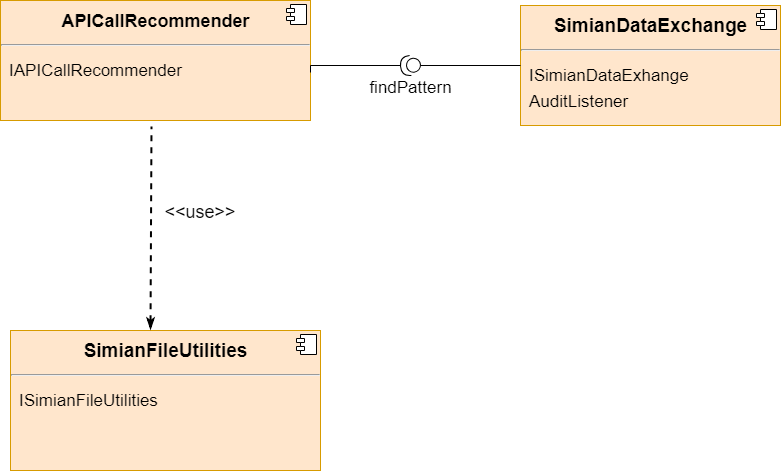
\includegraphics[width=12cm,height=12cm,keepaspectratio]{images/Component.png}
\centering
\caption{Component diagram}
\label{fig:cmd}
\end{figure}

\subsection{CLAMS adaptation}
Regarding the CLAMS output, we describe the original structure as well as the necessary modification to integrate it in our approach. The authors, differently from other works, provide the complete source code and commands to set up the entire environment to have CLAMS working on Linux . CLAMS is written in Python and uses srcXML and Astyle to produce XML files and to formatter in a human-readable way the code respectively, but as claimed by the authors, there is no really constrain about the technologies to use in case of a new implementation. As input, CLAMS takes two kind of files: client files, that represent the real project on Github related to the dataset that authors use for evaluation phase while example files are used as training set. All these files are collected in a folder, that CLAMS loads by getting the path. Moreover, there is a namespace file that identify the name of classes used in the clients and example files by using their complete namespaces such as org.codehaus.jackson. The last input used by the main.py file, that is used to initialise the platform, is the list of methods that are represented by an ARFF(Attribute-Relation File Format) file \cite{https://www.cs.waikato.ac.nz_last_nodate}, used in the machine learning domain. It is an ASCII text file that describes a list of instances sharing a set of attributes, specified in the header section. In our case, the attributes are the method declaration (the caller) and the method invocations (the calls). 
If we want to add some other libraries with respect to the original dataset (MQTT-Json projects), we need to replicate the same structure for CLAMS; to do this, we found on Github several projects related to this libraries and produce the ARFF files using Rascal, as we will see in the validation section
\newline
There is a phase of preprocessing in which CLAMS extracts API call and their AST using JDT utilities and represent them in xml using srcXML. The core of the project is the snippet generator module (represented by summarise.py file) that takes as input a source code file (java in this case) and using srcXML they first replace literals with xml types and delete comment. Then , they separate the API code from code that doesn't contain API call and highlights the variable in local scope of API. Finally, the code without API call is removed and Clams add some comments near the API statement and needed variables. Notice that their approach considers also the classical statement like if-else structure as a part of API statement. For clustering, they use both HDBSCAN and k-medoids algorithm that are quite similar and differs only in the precision of the returned snipped (HDBSCAN is more accurate but k-medoids covers more methods). For both of them, the authors import Python libraries that implement these algorithm quite well and we can switch the algorithm by change the parameter in the main.py. Moreover, they have the file ranking.py to order the generated snippet. The rank is based on the example files that contains a sequence of API call; if the sequence within the file is a super-sequence of the sequence of snippet that we considered, so this snippet is supported, and its rank is increased. In the result folder, CLAMS put the library that we want to analyze, the methods, the source file (both in .java and xml format), some JSON file that represent all information about a method (class, package, rank, id) and the arff file related to the library. \newline
For the integration step in our platform, it is necessary to slightly modify the original approach to have better results. In particular, if we use the pattern of CLAMS as they are, there are some bias because, through srcML, CLAMS substitutes the literals with its own type and Simian is not able to detect them as cloned code, even using all available options regarding the code. So, to avoid this situation, we must modify the function that substitute literals, putting some default value instead of srcML types. This modification doesn't affect the validity and accuracy of extracted path because is just a matter of modify literals with another and allow Simian to avoid bias in the code cloning analysis.

\subsection{API recommendations}
At the end of these preparatory phases, we describe now the core of this project, the API recommendations. Once the Simian is launched as we described, it performs the detection of code cloning activity on the CLAMS patterns files and the developer's code snippet. The typical scenario is depicted by the use case diagram in Figure 6, in which the developer asks for recommendations.


\begin{figure}[H]
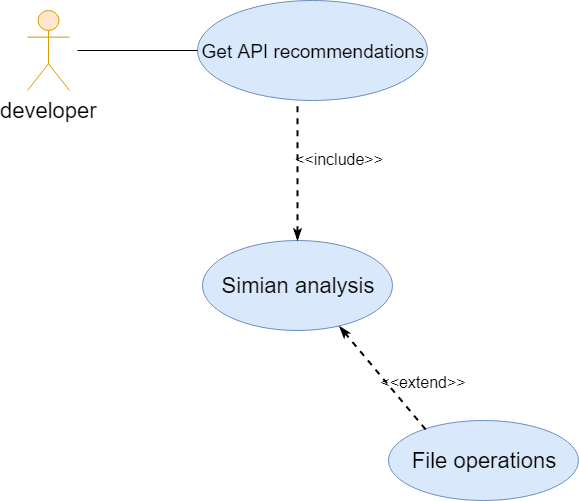
\includegraphics[width=10cm,height=10cm,keepaspectratio]{images/Usecase.png}
\centering
\caption{Use case scenario}
\label{fig:cmd}
\end{figure}

Notice that the notion of cloned code depends on the options that we have selected and turn on: the mandatory options to enable is the threshold, that set the minimum line of code in commons, reportDuplicateText, otherwise we couldn't show and manipulate the result and language that is Java because we analyze projects related to it. Without this options, Simian gives us only the fingerprints that represent the source coordinates of the files, that are not significant for our aims. So, to have a better representation, we have put the results in a wrapper class that represent the Pattern object in which we have all attributes to describe in the right manner the recommendation. Other options, such as the strings, identifiers or modifiers that should be introduced in the comparison, can be enable with respect to the level of cloning that we want to reach. To find useful results, it is necessary to set at least ignoreIdentifiers, ignoreIdentifierCase, ignoreLiterals, ignoreVariableName, ignoreNumbers and ignoreModifiers because Simian goes beyond the developer personal implementations and looking only for the structure of the code, in order to use the concept of pattern in a more effective way. Based on these options, Simian applies the proper transformations on the original textual code in order to perform the comparison. In this way, we are able to create a clone pairs to detect the similarities fixed by the options. \\
Furthermore, Simian compares the pair developer' snippet - pattern because some CLAMS pattern includes some duplicated lines of code and this can bring some bias. Once we load the files, the check is performed and the results that include lines of code, name of pattern file and time to perform the comparison and put all in the wrapper class mentioned before.
At the end of this step, we have the patterns (a complete one or only partial) that the developer is start to implement and we can discard it from the comparison, as the developer is not interested to see what he have done so far. Moreover, new pattern can introduce something new or suggest an alternative implementation for the developer. The last step is remove the duplicated line of code from the suggested pattern and show to the developer only the novel part, in form of some that integrate his code or completely new pattern, related of course to the APIs that he is implementing. About the ranking, we order the pattern by considering the number of cloned lines, so the first pattern is the contains more duplicated lines rather than second and so on. The rank phase is simply performed on the SimianPattern object that we produce as output. All the steps are summarized in the Sequence Diagram below.

\begin{figure}[H]
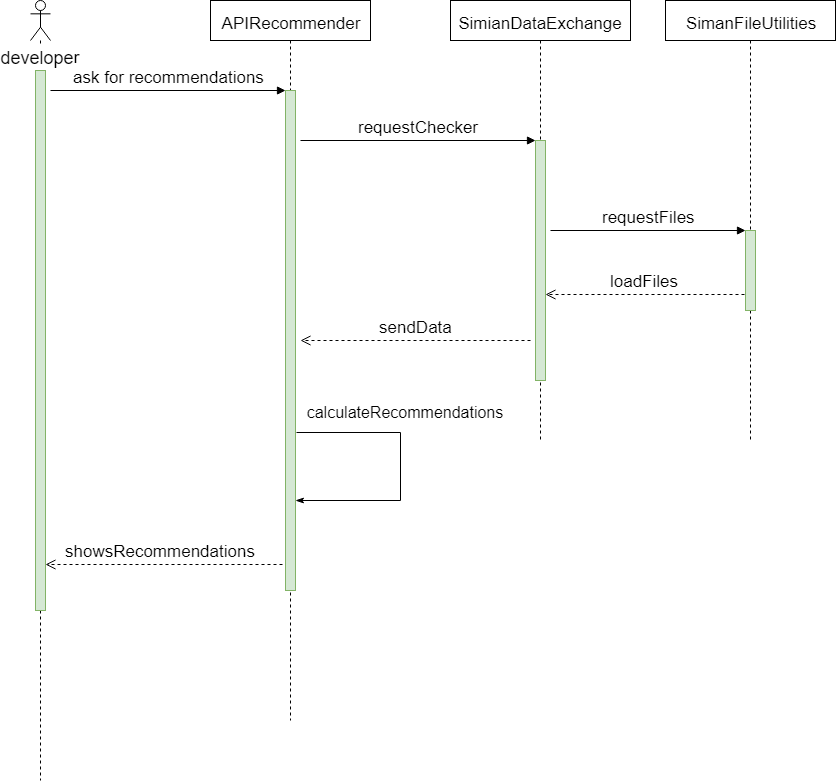
\includegraphics[width=12cm,height=14cm,keepaspectratio]{images/Sequence.png}
\centering
\caption{Sequence diagram }
\label{fig:cmd}
\end{figure}


In the example below, related to MQTT paho library, we have extracted the method publish() from the developer's file with Java Parser and run Simian on it.  The last columns shows two top rank CLAMS patterns related to it.
\vspace{5mm}

Developer's original file
\begin{lstlisting}
package org.eclipse.paho.sample.mqttv3app;
import java.io.IOException;
import java.sql.Timestamp;
import org.eclipse.paho.client.mqttv3.IMqttDeliveryToken;
import org.eclipse.paho.client.mqttv3.MqttCallback;
import org.eclipse.paho.client.mqttv3.MqttClient;
import org.eclipse.paho.client.mqttv3.MqttConnectOptions;
import org.eclipse.paho.client.mqttv3.MqttException;
import org.eclipse.paho.client.mqttv3.MqttMessage;
import org.eclipse.paho.client.mqttv3.persist.MqttDefaultFilePersistence;

public class Sample implements MqttCallback {		
   	public Sample(String brokerUrl, String clientId, boolean cleanSession, boolean quietMode, String userName, String password) throws MqttException {    	
    		try {    		
	    	conOpt = new MqttConnectOptions();
	    	conOpt.setCleanSession(clean);
	    		if(password != null ) {
	    	  		conOpt.setPassword(this.password.toCharArray());
	    		}
	    		if(userName != null) {
	    	  		conOpt.setUserName(this.userName);	   
	    		}    		
			client = new MqttClient(this.brokerUrl,clientId, dataStore);		
	    	client.setCallback(this);
	    	
		} catch (MqttException e) {
			e.printStackTrace();
			log("Unable to set up client: "+e.toString());
			System.exit(1);
		}
    }

    public void publish(String topicName, int qos, byte[] payload) throws MqttException {
    	
    	// Connect to the MQTT server
    	log("Connecting to "+brokerUrl + " with client ID "+client.getClientId());
    	client.connect(conOpt);
    	log("Connected");   	
    	String time = new Timestamp(System.currentTimeMillis()).toString();
    	log("Publishing at: "+time+ " to topic \""+topicName+"\" qos "+qos);    
   	MqttMessage message = new MqttMessage(payload);
    	message.setQos(qos);     
    	client.publish(topicName, message);    	
    	// Disconnect the client
    	client.disconnect();
    	log("Disconnected");
    }
    
  
    public void subscribe(String topicName, int qos) throws MqttException {    	    
    	client.connect(conOpt);
    	log("Connected to "+brokerUrl+" with client ID "+client.getClientId());    
    	log("Subscribing to topic \""+topicName+"\" qos "+qos);
    	client.subscribe(topicName, qos);
    	// Continue waiting for messages until the Enter is pressed
    	log("Press <Enter> to exit");
		try {
			System.in.read();
		} catch (IOException e) {
			//If we can't read we'll just exit
		}		
		// Disconnect the client from the server
		client.disconnect();
		log("Disconnected");
    }
}
\end{lstlisting}


\vspace{5mm}
\newpage
Extracted method:
\begin{lstlisting}

   // Connect to the MQTT server
    log("Connecting to " + brokerUrl + " with client ID " + client.getClientId());
    client.connect(conOpt);
    log("Connected");
    String time = new Timestamp(System.currentTimeMillis()).toString();
    log("Publishing at: " + time + " to topic \"" + topicName + "\" qos " + qos);
    // Create and configure a message
    MqttMessage message = new MqttMessage(payload);
    message.setQos(qos);
    // Send the message to the server, control is not returned until
    // it has been delivered to the server meeting the specified
    // quality of service.
    client.publish(topicName, message);
    // Disconnect the client
    client.disconnect();
    log("Disconnected");
 \end{lstlisting}
\vspace{5mm}

\begin{minipage}[t]{0.5\textwidth}
\begin{lstlisting}
CLAMS pattern #1

{
    String pubTopic;
    MqttClient pubClinet;
    String payload;
    int qos;
    pubClinet = new MqttClient(url, clientId);
    pubClinet.setCallback(this);
    pubClinet.connect();
    MqttMessage message = new MqttMessage(payload.getBytes());
    pubClinet.publish(pubTopic, message);
    pubClinet.disconnect();
}
\end{lstlisting}
\end{minipage}
\begin{minipage}[t]{0.5\textwidth}

\begin{lstlisting}
CLAMS pattern #2

{
    String topicName;
    MqttAsyncClient client;
    MqttConnectOptions conOpt;
    String brokerUrl;
    byte[] payload;
    int qos;
    log("a string"+brokerUrl + "a string"+client.getClientId());
    IMqttToken conToken = client.connect(conOpt,null,null);
    log("a string"+System.currentTimeMillis()+ "a string"+topicName+"a string"+qos);
    IMqttDeliveryToken pubToken = client.publish(topicName, message, null, null);
    pubToken.waitForCompletion();
    IMqttToken discToken = client.disconnect(null, null);
    discToken.waitForCompletion();
}

	
\end{lstlisting}
\end{minipage}
\newline
In particular, the two extracted recommendations show two possible use of the object MqttMessage that the developer declare in the publish method. The first recommendation add an MqttClient while the second use the interface IMqttDeliveryToken as a different way to send the mqtt message. Of course, the number of recommendation is strongly related to the length of the method and how many lines Simian can detect in its textual analysis. This example is just to show the expected output after running our approach. In general, given a project that uses different libraries, with this approach we are able to recommend patterns of whatever libraries that the user are interested to develop. As mentioned before, recommendations are at level of code snippet, that provide a concrete and immediate hint. As we choose CLAMS for the second element of the clone pair, we are not able to provide tutorial or complete application as recommendation, because only the patterns are available for this purpose. \\
We can support almost the dataset of CLAMS, because the authors provides all necessary files on Github to have the patterns. The table below summarize the dataset with supported libraries and the number of patterns extracted by CLAMS. As developer's file, we choose main classes of Github projects related to the libraries that we want to support with the code cloning approach. We also include the MQTT and Json libraries missing in the CLAMS original dataset to cover different contexts with respect to the CLAMS approach and introduce novelty in this field. Notice that quality of recommendations depends first of all on the blocks in the developer's file that Simian is able to detect in the patterns provided by CLAMS. More patterns means more support for the library and this bring more API recommendations at the end of the process. An other aspect to taking into account is that Simian analyse the duplicated blocks of code and maybe some methods invocations that are not in the correct sequence are discarded automatically from the final recommendation. \\
In next section we set up an evaluation framework  by using part of the dataset of CLAMS (as we have already the patterns used by Simian for the comparison). We do this as a double check validation because Simian not have a postprocessing phase as we said in the related section and we need a comparison that goes beyond the lexical one in order to apply the metrics. Moreover, we will compare the Simian results with PAM, already described in the existing approach section.




